\documentclass{article}
\usepackage[utf8]{inputenc}
\usepackage{natbib}
\usepackage{graphicx}
\usepackage[utf8]{inputenc}
\usepackage{comment} % enables the use of multi-line comments (\ifx \fi) 
\usepackage{fullpage} % changes the margin
\usepackage{hyperref}
\usepackage{amsmath}
\usepackage{mathtools}
\usepackage{booktabs} % For formal tables
\usepackage{listings}
\begin{document}
\noindent
\large\textbf{Software Engineering Process} \hfill \textbf{Amit Sachdeva} 

\normalsize Topic: Final Deliverables \hfill \textbf{40084627} 

Prof. P. Kamthan \hfill Due Date: 12/July/2019
\begin{center}
    \section*{Problem 1}
\end{center}
\section{Introduction} 
\textbf{Gamma Function: } It is commonly referred as factorial function for complex numbers. It is derived by Daniel Bernoulli. The gamma function $\gamma(z)$ is defined for all complex values of z larger than zero. Complex number can be consist of real and imaginary number, like $z = a + ib$ in which a and b can real numbers. A complex number is typically written in the form where sigma σ is the real part and it is the imaginary part.
\begin{figure}[h!]
\centering
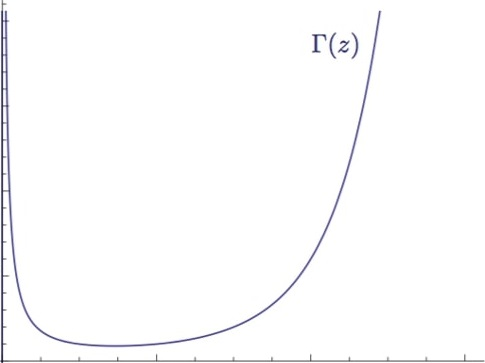
\includegraphics[scale=0.4]{gamma1}
\caption{The Universe}
\label{fig:Gamma Function}
\end{figure}
\section{Overall Description} 
This is a project based on gamma function in which we are making calculator for gamma value. User can insert any real value and expect real value except on boundary conditions.

\section{Stakeholders} 
\textbf{Users 1:} This function is mostly used in physics calculations. So, most important stakeholders are scientists for their calculations.
\newline
\textbf{Users 2:} This function is also used in basic maths calculations or any analytically field. 



\section{Related to Function}
\subsection{Formulas}
\begin{itemize}
\item \textbf{Formula1: } $  \Gamma \left( x \right) = \int\limits_0^\infty {s^{x - 1} e^{ - s} ds} \enspace \forall \enspace Re(x)>0$
\item \textbf{Formula2: } $  \Gamma \left( 1/2 \right) = \sqrt{\pi}$
\item \textbf{Formula3: } $  n! = n*(n-1)!$
\item \textbf{Formula4: } $  \Gamma \left( x \right) = x\Gamma \left( x-1\right) $
\item \textbf{Formula5: } $  \Gamma \left( 0 \right) = undefined $
\end{itemize}

\subsection{Domain of Function}
$\forall$ Real numbers excluding all negative integers \\
$(-\infty, \infty) - Z^{-}$

\subsection{Co domain of Function}
\begin{itemize}
\item It ranges from $(-\infty, \infty)$
\item For positive integers, we returns integer value as normal factorial
\item For other real numbers, we use integral function.
\end{itemize}

\section{Requirements/Constraints of Function}
\subsection{Requirements}
\begin{itemize}
\item \textbf{Req1}: For \textbf{Large input} in positive value, it will return infinity as \textbf{Const3}.
\item \textbf{Req2}: For \textbf{negative input} $\forall x<0 $, \textbf{Function} will return \textbf{real number} response, keeping in mind \textbf{Const1} and \textbf{Const2}
\item \textbf{Req3}: For \textbf{$x=0$}, \textbf{Function} will return \textbf{undefined}, keeping in mind \textbf{Const1}
\item \textbf{Req4}: For \textbf{$Re(x) > 0$}, \textbf{Function} will return positive real value, keeping in mind \textbf{Const1}
\end{itemize}

\subsection{Constraints}
\begin{itemize}
\item \textbf{Const1}: For Input, types must be Integer, Double, Float data types
\item \textbf{Const2}: We cannot \textbf{input} value of \textbf{non negative integers}
\item \textbf{Const3}: We cannot input the value large positive number as it will return infinity as a programming language constraint
\end{itemize}

\section{References}
\begin{itemize}
\item https://www.ncbi.nlm.nih.gov/pmc/articles/PMC4247832/
\item https://medium.com/cantors-paradise/the-riemann-hypothesis-explained-fa01c1f75d3f
\end{itemize}
\end{document}
